% !TeX encoding = ISO-8859-1
\chapter{nRF52DK}
\label{chap:nrf52dk}

\begin{figure}[h]
	\centering
	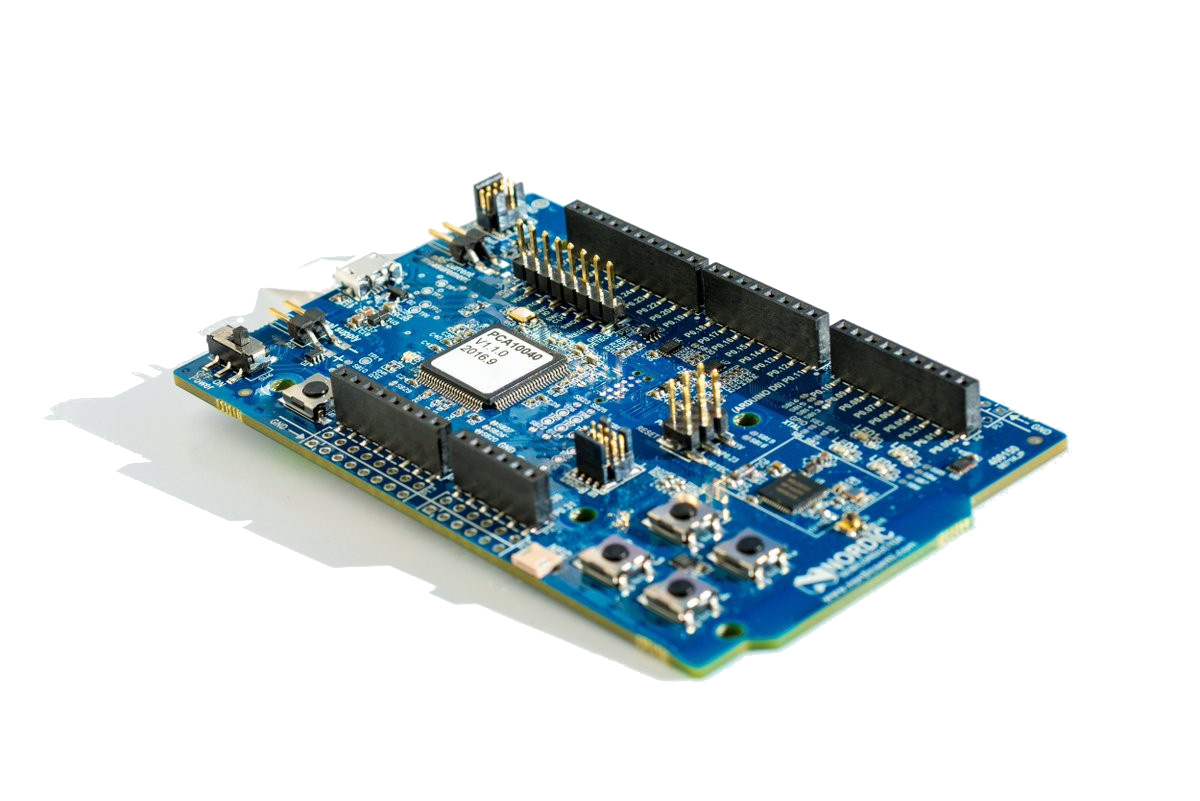
\includegraphics[width=1.0\linewidth]{bilder/nrf52_board.jpg}
	\caption{Das nRF52 Development Kit}
	\label{fig:devkit}
\end{figure}

Das nRF52 DK ist eine single-Board Entwicklungsplatform welche f�r die Verwendung von \ac{BLE}, ANT, und propriet�ren 2.4GHz Protokollen ausgelegt ist. Herzst�ck des Kits ist das nRF52832 \ac{SoC}.

Die Header sind kompatibel mit allen Arduino Shields des Revisionsstandards 3 was das Kit enorm erweiterbar macht. Weiter besteht die M�glichkeit eine mitgelieferte NFC-Antenne anzuschliessen um NFC-Tags zu lesen. Alle GPIOs sind via Header herausgef�hrt. Zus�tzlich verf�gt das Board �ber 4 LEDs und 4 Taster. 

\newpage

\section{Technische �bersicht}

\begin{figure}[h]
	\centering
	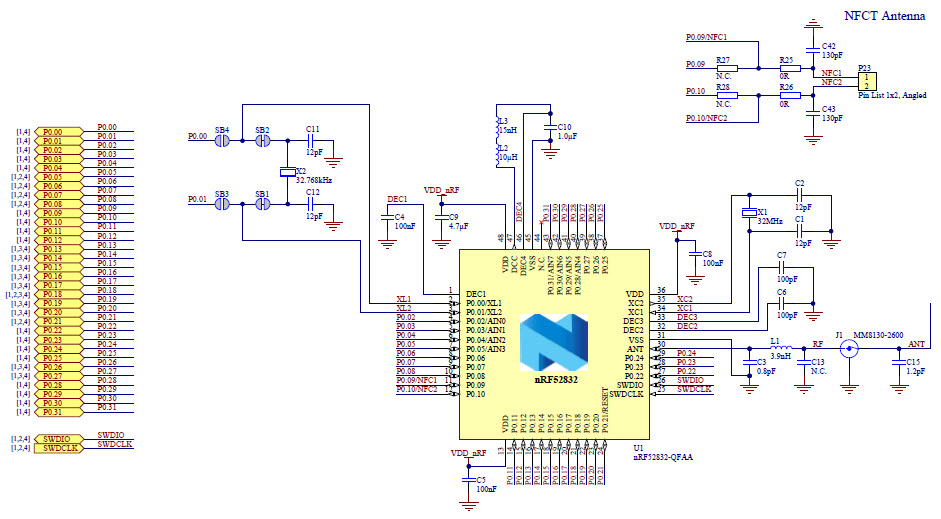
\includegraphics[width=1.0\linewidth]{bilder/nrf52_schematic.jpg}
	\caption{Schema des nRF52DKs aus der Dokumentation von Nordic entnommen}
	\label{fig:schematic}
\end{figure}

\section{Installation der GNU ARM Embedded Toolchain}

Um die Funktion aller Tools und der SDK zu gew�hrleisten, sollten folgende Installationen ausschliesslich in der hier beschriebenen Reihenfolge ausgef�hrt werden. Da sich die Installation unter Ubuntu und Arch Linux unterscheiden, sind im nachfolgenden beide Varianten dokumentiert. 

Um die Software auf dem Hostsystem f�r das nRF52DK kompilieren zu k�nnen, ben�tigen wir eine sogenannte crosscompiler-toolchain. F�r ARM basierte Controller ist hier die erste Wahl die gnu-arm-none-eabi Toolchain. Sie l�sst sich von folgender Seite beziehen:

\url{https://launchpad.net/gcc-arm-embedded/+download}

Es gilt darauf zu achten, die neueste Version zu verwenden und sich zu notieren, welche Version heruntergeladen wurde, da diese sp�ter im Makefile angegeben werden muss. Die Software sollte im Verzeichnis /opt installiert werden. Die Binaries sollten mit den n�tigen Rechten ausgestattet werden. Weiter empfiehlt es sich symbolische Links zu generieren, um die Programme systemweit sichtbar zu machen.

Die Befehle dazu lauten:

\begin{lstlisting}[style=BashInputStyle]
    tar -xf gcc-arm-none-eabi-linux.tar.bz2 /opt/gcc-arm-none-eabi-tools
    ln -s /opt/gcc-arm-none-eabi-tools/bin/* /usr/local/bin/
\end{lstlisting}

Wichtig: Unter Arch Linux sollte unbedingt die aktuellste Version im Community Repository verwendet werden. Die gew�nschte Software l�sst sich wie folgt installieren:

\begin{lstlisting}[style=BashInputStyle]
    pacman -S community/arm-none-eabi-binutils
    pacman -S community/arm-none-eabi-newlib
    pacman -S community/arm-none-eabi-gcc
    pacman -S community/arm-none-eabi-gdb
\end{lstlisting}


\section{Installation der nordic SDK}

Nordic Semiconductor verf�gt �ber ein Software Archiv von welchem alle ben�tigte Software bezogen werden kann. Das Archiv befindet sich unter folgendem Link:

\url{https://www.nordicsemi.com/eng/Products/Bluetooth-low-energy/nRF52-DK#Downloads}

Um mit dem nRF52 Entwicklungskit arbeiten zu k�nnen, ben�tigen wir folgende Softwarepakete:

\begin{enumerate}
    \item nRF5 SDK Zip File
    \item nRF5x-Command-Line-Tools-Linux64
\end{enumerate}

Im ersten Paket befinden sich alle Files, welche zur Entwicklung von Software auf dem nRF52dk notwendig sind. Darunter Makefiles, Linkerskripte und auch Beispielcode.
Im zweiten Paket befinden sich die Command-Line-Tools, welche es uns erm�glichen �ber die Kommandozeile mit dem nRF52 Entwicklungskit zu kommunizieren. Das wichtigste Tool ist nrfjprog, welches kompilierte Programme auf das Board hochladen kann.

Die SDK sowie die Command-Line-Tools sollten auf dem System unter dem Ordner /opt installiert werden und mit den n�tigen Berechtigungen versehen werden. Ebenfalls sollten die Programme in einen Ordner gelinkt werden, welcher im Systempfad angegeben ist.

Die Befehle dazu lauten:
\begin{lstlisting}[style=BashInputStyle]
    tar -xf nRF5x-Command-Line-Tools-Linux64.tar /opt/
    ln -s /opt/nrfjprog/nrfjprog /usr/bin/nrfjprog
    ln -s /opt/mergehex/mergehex /usr/bin/mergehex
\end{lstlisting}

Unter Arch Linux lassen sich die Command Line Tools auch �ber das Arch User Repository beziehen. Dazu kann man den Pacman Wrapper ''yaourt'' verwenden:

\begin{lstlisting}[style=BashInputStyle]
    yaourt -S aur/nrf5x-command-line-tools 
\end{lstlisting}

\section{Installation des SEGGER JLink Debuggers}

Die Software von SEGGER, welche f�rs Debuggen gebraucht wird, findet man unter folgendem Link:

\url{https://www.segger.com/downloads/jlink}

Das Paket ''J-Link Software and Documentation Pack'' enth�lt verschiedene Programme. Die Wichtigsten davon sind der JLinkCommander und der JLinkGDBServer. �ber den Commander l�sst sich die CPU des nRF52 vollst�ndig via JTAG oder SWD Schnittstelle kontrollieren. Der JLinkGDBServer stellt auf dem Localhost einen Socket unter Port 2331 zur Verf�gung, auf welchen man sich mit GDB verbinden kann.

Die JLink Toolchain sollte auf dem System unter dem Ordner /opt installiert werden und mit den n�tigen Berechtigungen versehen werden. Die Programme sollten mittels symbolischen Links in einen Ordner gelinkt werden, welcher im Systempfad angegeben ist.

\begin{lstlisting}[style=BashInputStyle]
    mkdir /opt/SEGGER/JLink
    tar -xzf JLink_Linux_{VERSION}.tar.gz /opt/SEGGER/JLink
    ln -s /opt/SEGGER/JLink/JLinkExe /usr/bin/JLinkExe
    ln -s /opt/SEGGER/JLink/JLinkGDBServer /usr/bin/JLinkGDBServer
\end{lstlisting}

SEGGER bietet auch ein Debianpaket an. Dieses kann auf Systemen, welche �ber den Paketmanager DPKG verf�gen mittels \verb|dpkg -i JLink_linux.deb| installiert werden. Dadurch entf�llt obiger Installationsaufwand.\newline

Unter ArchLinux l�sst sich die Software auch aus dem Arch-User-Repository installieren, der Befehl dazu lautet:
\begin{lstlisting}[style=BashInputStyle]
    yaourt -S aur/jlink-software-and-documentation
\end{lstlisting}

\section{Verwendung des JLinkGDBServers}

Der folgende Befehl beschreibt das Starten des GDBJLinkServers von SEGGER. 

\begin{lstlisting}[style=BashInputStyle]
    JLinkGDBServer -Device nRF52832_xxAA -If SWD -Speed 4000 -Autoconnect 1
\end{lstlisting}

Der Server startet einen lokalen Socket und ist unter Port 1234 erreichbar.
Nachdem \ac{GDB} gestartet wurde, l�sst sich �ber folgenden Befehl eine Verbindung mit dem Server herstellen:

\textbf{(gdb) target remote localhost:1234}

Alternativ kann auch eine Konfigurationsdatei f�r GDB angelegt werden. Dazu erstellt man im Home-Verzeichnis eine Datei mit dem Namen .gdbinit. Um automatisch auf den lokalen Server zu verbinden ist lediglich die obere Zeile hinzuf�gen. 

\section{Verwendung von nrfjprog}

Nrfjprog ist Teil der Propriet�ren Softwarewerkzeuge der SDK von Nordic. Es unterst�tzt das Flashen von Hex-Binarys �ber SWD oder JTAG. Der Funktionsumfang ist sehr gross, daher sei an dieser Stelle auch noch aufs Helpfile verwiesen.

Um eine bereits kompilierte Beispielapplikation auf das nrf52 Board zu laden sind folgende Befehle in dieser Reihenfolge auszuf�hren.

\begin{lstlisting}[style=BashInputStyle]
    nrfjprog --eraseall -f nrf52
    nrfjprog --program outdir/nrf52_pca10040/zephyr.hex -f nrf52
    nrfjprog --reset -f nrf52
\end{lstlisting}

Zeile 1 l�scht den aktuellen Inhalt des Flashspeichers auf dem SoC.\newline
Zeile 2 flasht ein neues Binary in den Flashspeicher des SoC.\newline
Zeile 3 Resetet den SoC, alternativ kann auch der Hardwarereset bet�tigt werden.\newline
